\section{GreyResNet18 encoder and projection head}
\label{app:greyresnet18_architecture}

\begin{figure}[H]
  \centering
  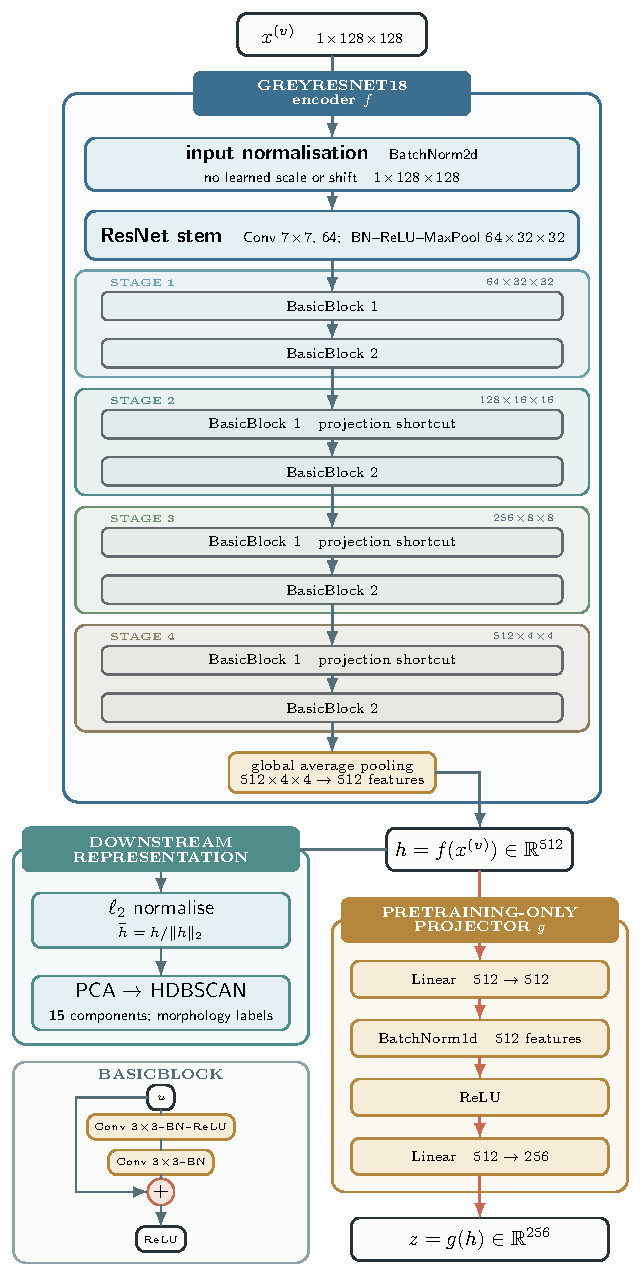
\includegraphics[
    width=\linewidth,
    height=0.72\textheight,
    keepaspectratio
  ]{img/greyresnet18_projector_architecture.pdf}
  \caption[GreyResNet18 encoder and projection head]{GreyResNet18 encoder and projection head used for contrastive
    pre-training, shown for one generic augmented view \(x^{(v)}\); both SimCLR
    views pass through the same encoder and projector parameters. In the
    ResNet stem, the \(7\times7\) convolution and max-pooling operation both
    use stride \(2\). The first BasicBlock of stages 2--4 halves the spatial
    resolution: its first \(3\times3\) convolution and its \(1\times1\)
    projection shortcut use stride \(2\), whereas the remaining BasicBlocks
    use stride \(1\) and identity shortcuts. Global average pooling is
    implemented by adaptive average pooling followed by flattening, producing
    the \(512\)-dimensional representation \(h\). The projection head \(g\) is
    used only during pre-training and maps \(h\) to the \(256\)-dimensional
    projection \(z\); it is discarded for downstream analysis.}
  \label{fig:greyresnet18_architecture}
\end{figure}

\clearpage
\section{Raw PCA--HDBSCAN cluster overview}
\label{app:hdbscan_cluster_overview}

Figures~\ref{fig:hdbscan_cluster_overview_first} and~\ref{fig:hdbscan_cluster_overview_second} show the raw groups used during manual inspection, with actual HDBSCAN labels \(-1,0,\ldots,58\). Table~\ref{tab:cluster_class_mapping} records their consolidation into the eleven morphology classes.

\begin{figure}[H]
  \centering
  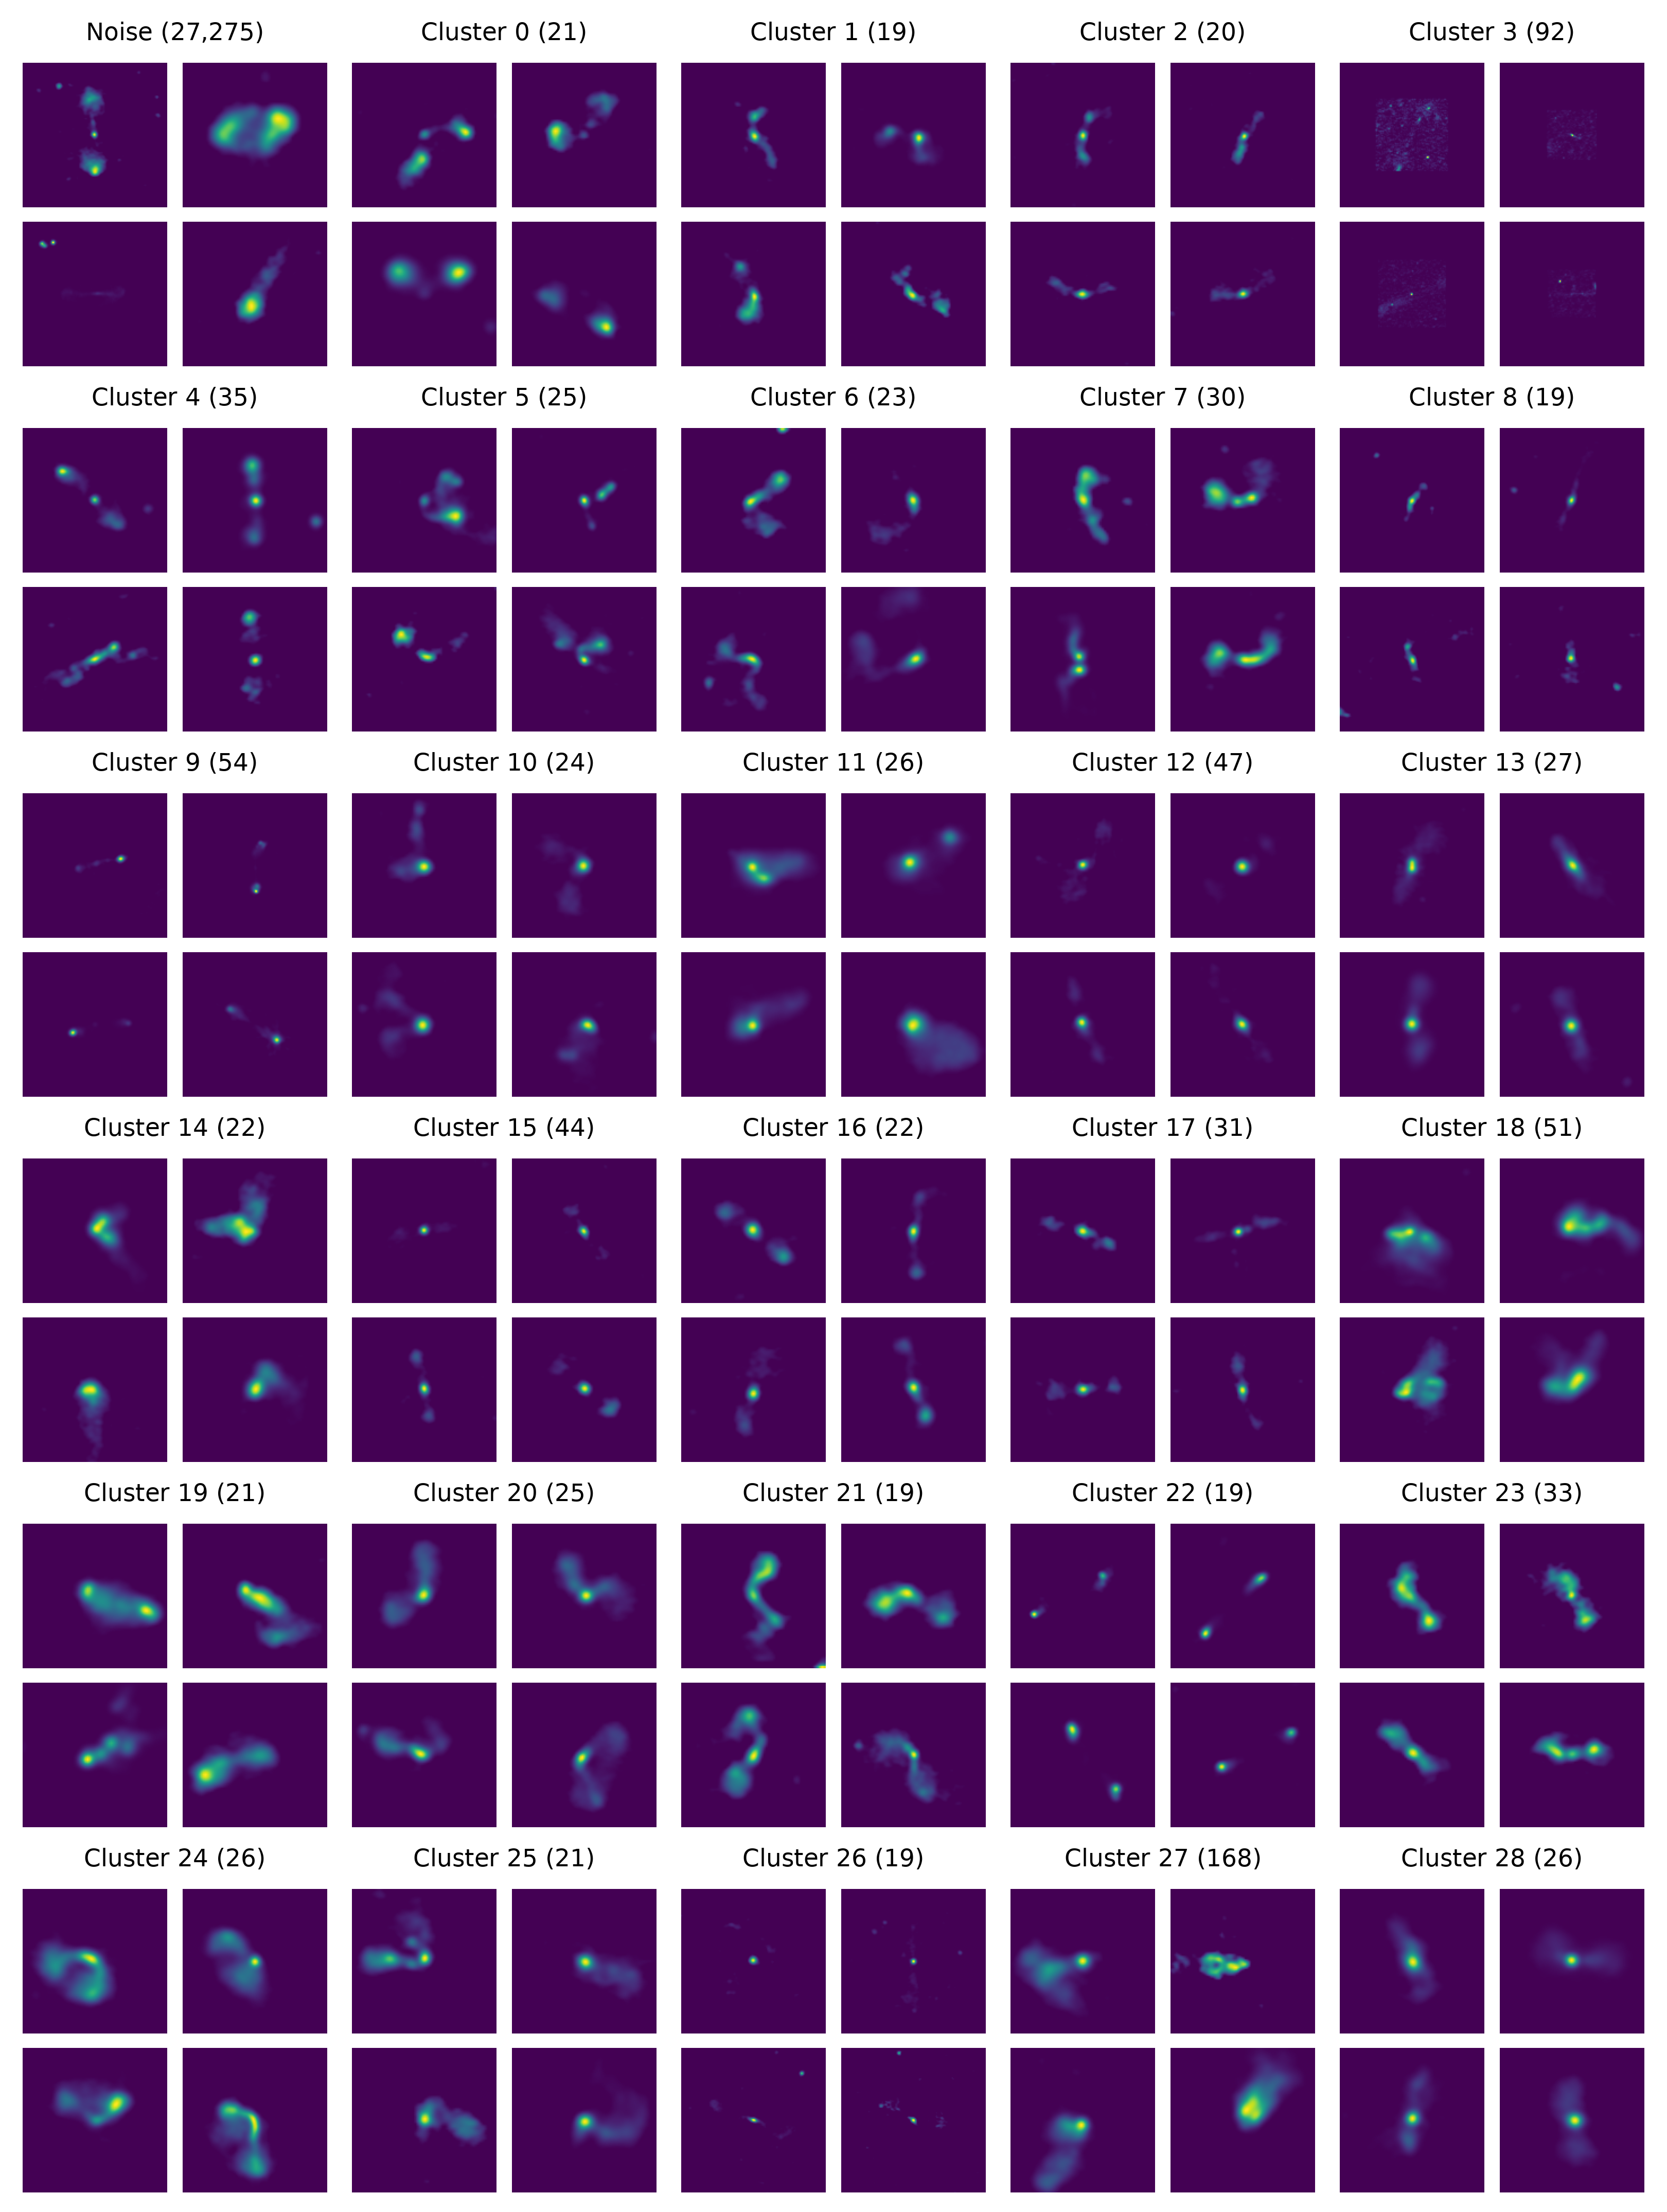
\includegraphics[width=\linewidth,height=0.73\textheight,keepaspectratio]{img/hdbscan_cluster_portrait_noise_28.png}
  \caption[HDBSCAN overview: noise and clusters 0--28]{Noise group \(-1\) and clusters 0--28, read left to right and top to bottom. Each group shows four examples; parentheses give its total membership.}
  \label{fig:hdbscan_cluster_overview_first}
\end{figure}
\clearpage
\begin{figure}[p]
  \centering
  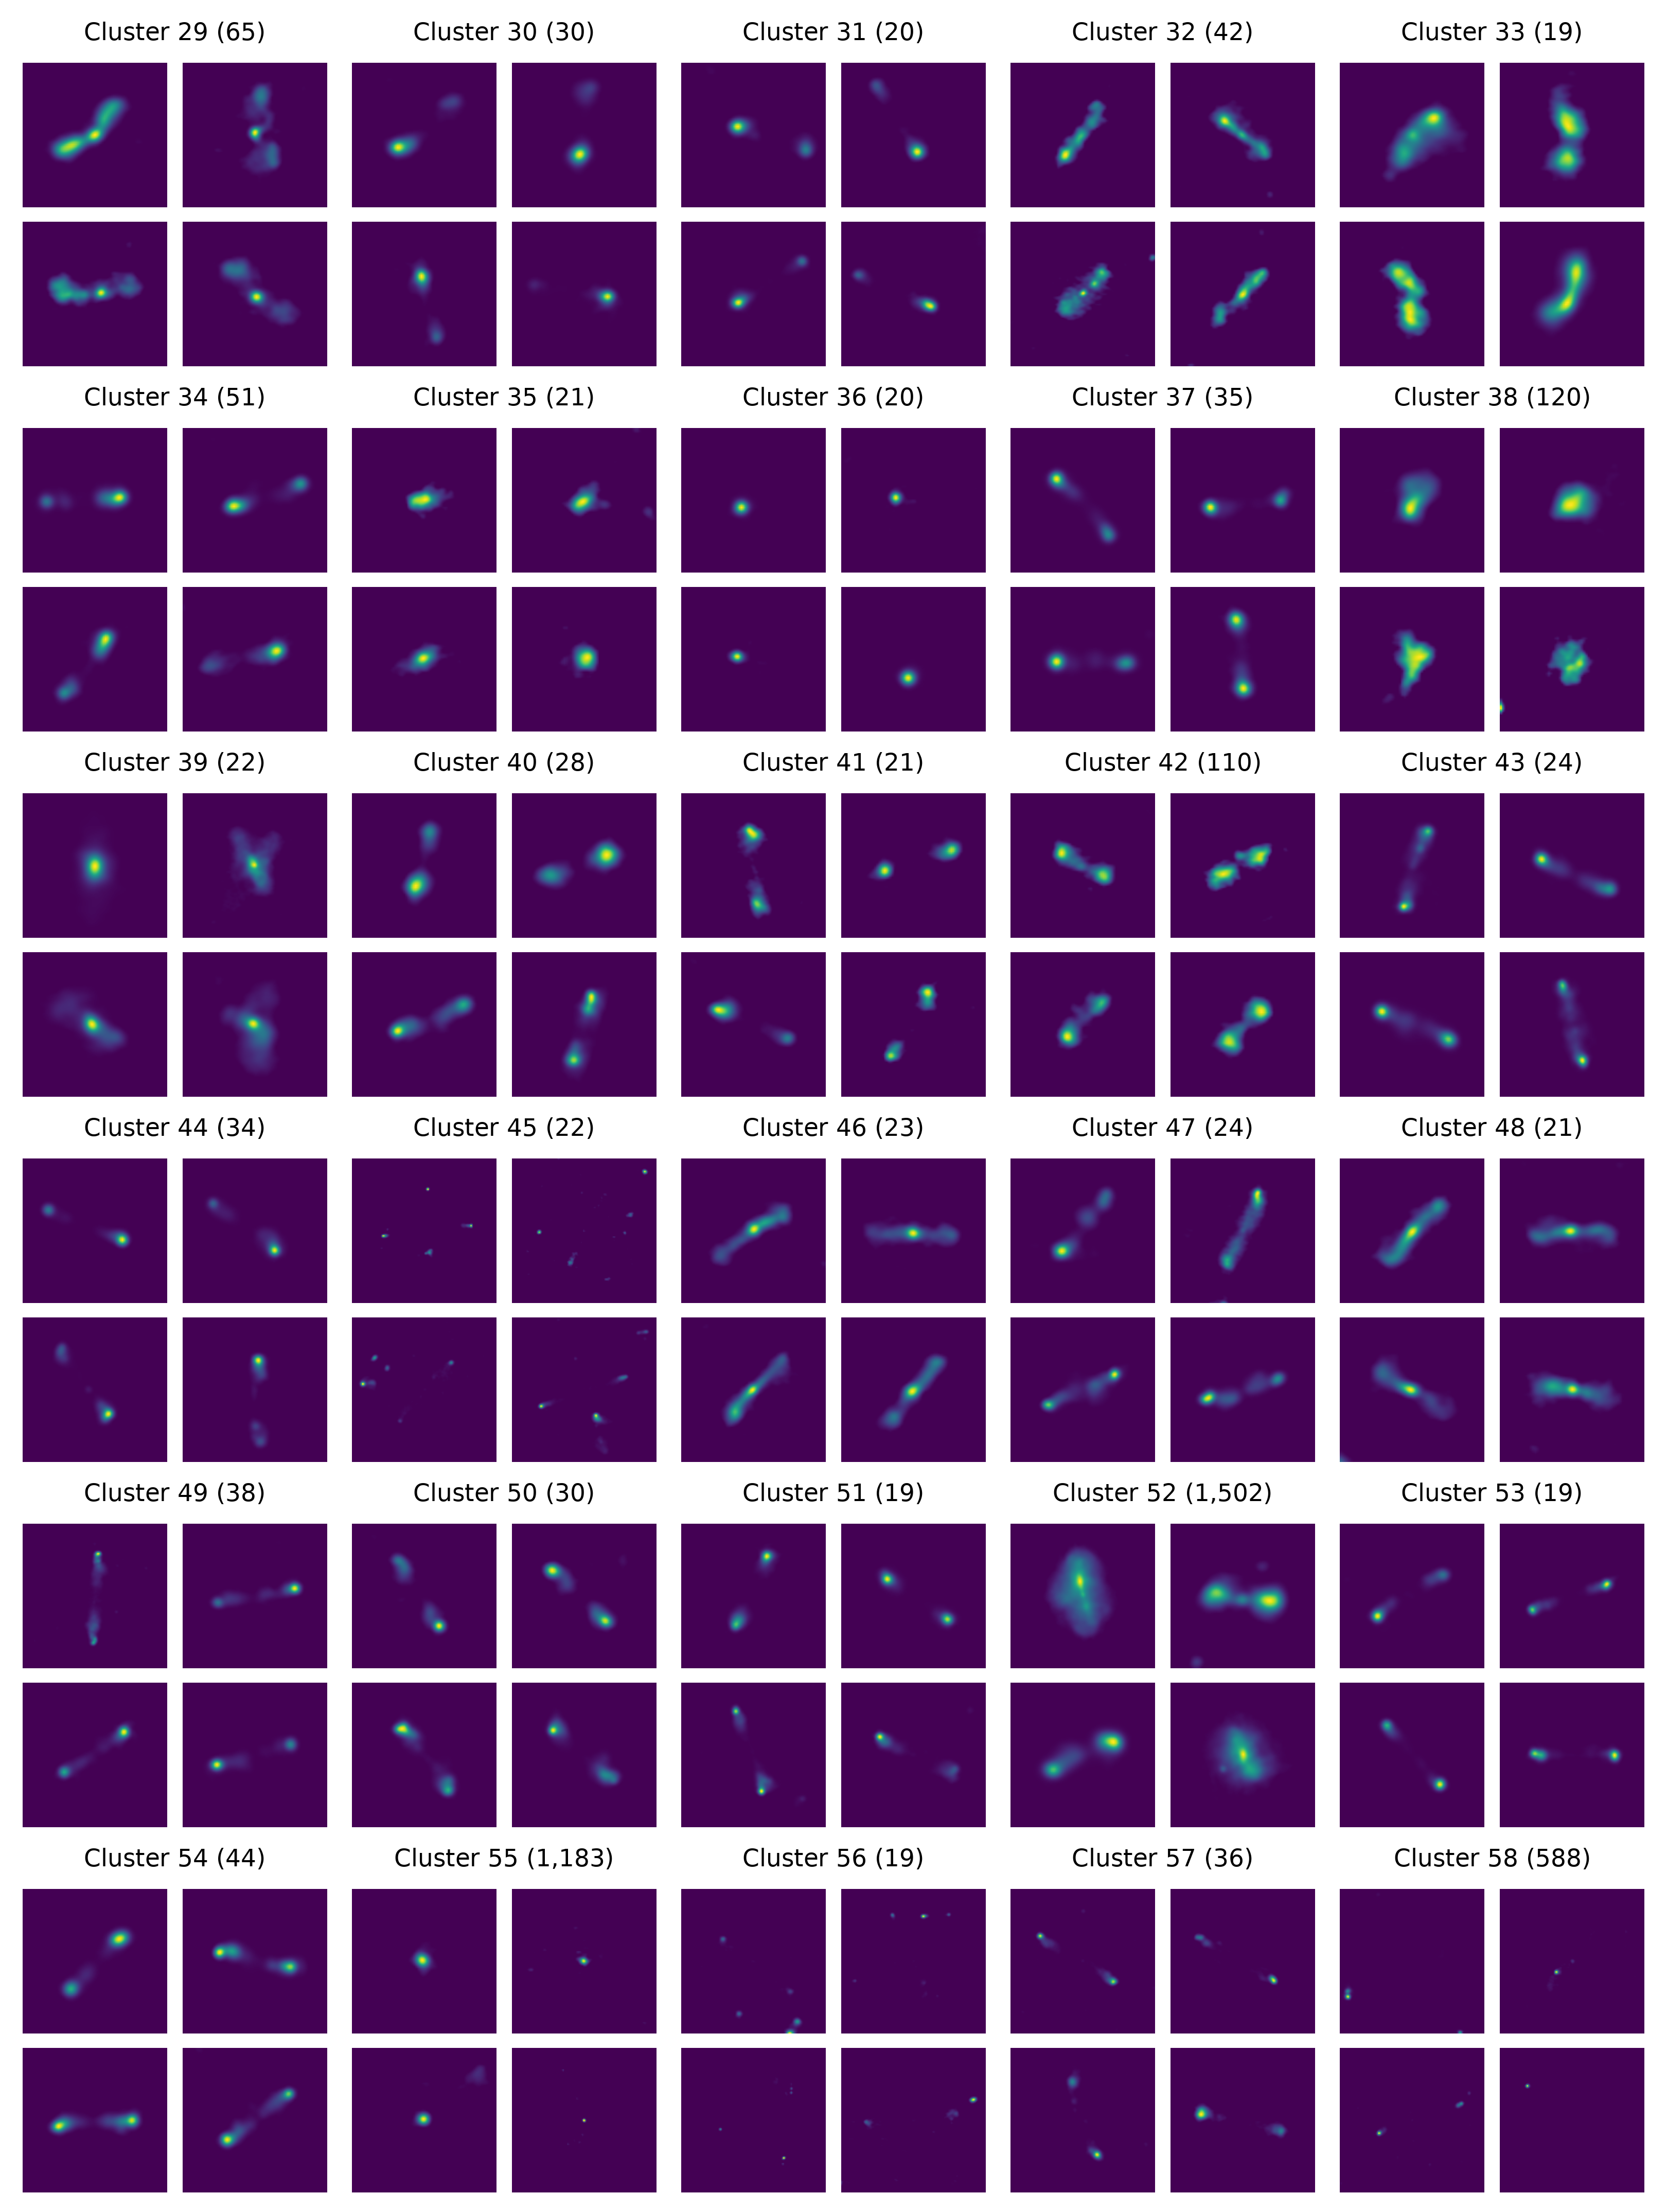
\includegraphics[width=\linewidth,height=0.83\textheight,keepaspectratio]{img/hdbscan_cluster_portrait_29_58.png}
  \caption[HDBSCAN overview: clusters 29--58]{Clusters 29--58, in the same format as Figure~\ref{fig:hdbscan_cluster_overview_first}.}
  \label{fig:hdbscan_cluster_overview_second}
\end{figure}
\clearpage

\begin{table}[H]
\centering
\small
\setlength{\tabcolsep}{4pt}
\begin{tabular}{@{}lp{0.48\linewidth}r@{}}
\toprule
Morphology class & Raw HDBSCAN labels & Sources \\
\midrule
Amorphous & 35 & 21 \\
ACJ & 11, 14 & 48 \\
Bright-core & 55 & 1\,183 \\
Centre-bright FRI & 2, 4, 8, 12, 13, 15, 16, 17, 26, 28, 46, 48 & 334 \\
Core-Displaced & 36 & 20 \\
Edge-bright FRII & 22, 30, 31, 34, 37, 40, 41, 42, 43, 44, 47, 49, 50, 51, 53, 54 & 546 \\
Hybrid & 23, 32 & 75 \\
Large FRII & 9, 57 & 90 \\
Spirals & 38 & 120 \\
Structured-Bent & 0, 1, 5, 6, 7, 10, 20, 21, 24, 25, 29 & 298 \\
Unresolved & 3, 45, 56, 58 & 721 \\
\midrule
Returned to unassigned & 18, 19, 27, 33, 39, 52 & 1\,783 \\
Original noise & \(-1\) & 27\,275 \\
\bottomrule
\end{tabular}
\caption[Raw-cluster consolidation into morphology classes]{Raw-cluster consolidation before SI-SSIM filtering. Every raw label occurs once; source counts sum to \(32\,514\).}
\label{tab:cluster_class_mapping}
\end{table}
